\section{Struttura delle memorie}
Le memorie hanno in generale diverse tipologie si strutture di controllo in base alla loro costruzione. La costruzione di una memoria non è universale, ciò è dovuto alla differente implementazione che tali memorie hanno a livello pratico. In una maniera più generale, le memorie possono essere suddivise in due categorie:
\begin{itemize}
    \item \textbf{Memorie statiche}: Le memorie statiche sono memorie che sono costruite tramite un insieme di transistor opportunamente collegati, non richiedono alcun tipo di sistema di refresh dei dati
    \item \textbf{Memorie dinamiche}: Le memorie dinamiche sono memorie che funzionano mediante effetti capacitivi. Pertanto richiedono che vi sia implementato un opportuno sistema di refresh
\end{itemize}
Tali memorie vengono utilizzate in base all'ambito di applicazione e alla velocità richiesta. Tali argomentazioni saranno affrontate nei capitoli appositi

\subsection{Memorie Dinamiche}
Le memorie dinamiche sono memorie che utilizzano gli effetti capacitivi per memorizzare l'informazione. Un esempio semplice di cella di memorizzazione di una memoria dinamica è osservabile alla figura [\ref{img:mem-dinamica}]. Come possiamo notare, la memorizzazione dipende fortemente dalla carica di un condenzatore, che quindi richiede di dover implementare un meccanismo di refresh. Tale meccanismo di refresh può essere fatto in vari modi, in base alle modalità di accesso ai dati della specifica memoria.

\begin{figure}
    \centering
    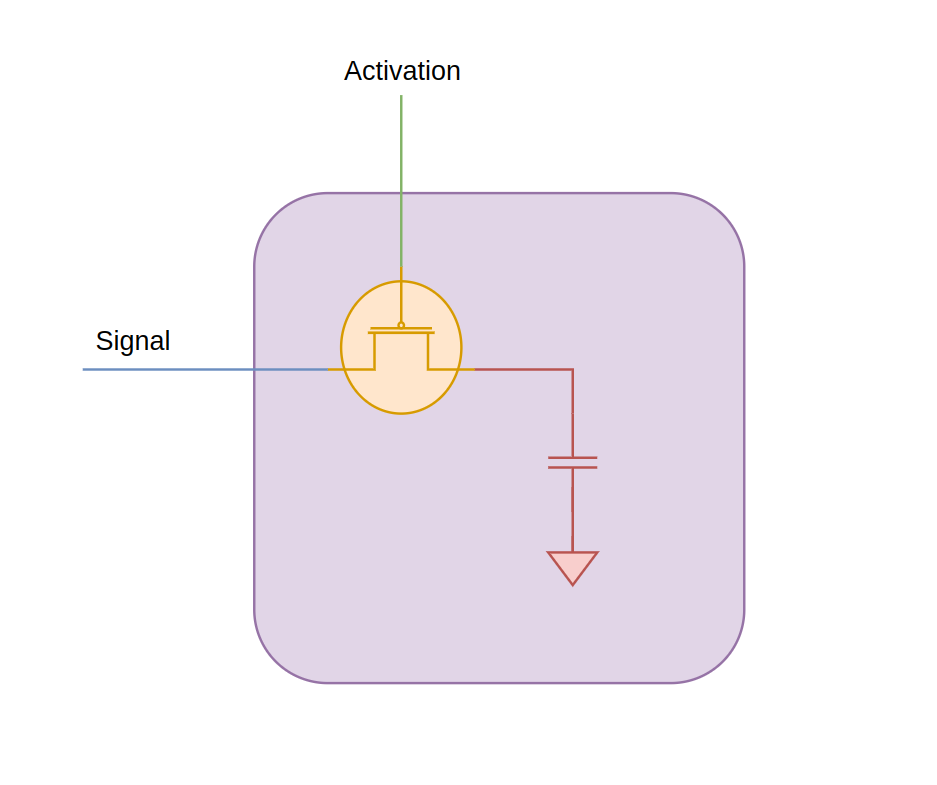
\includegraphics[width=.3\textwidth]{img/DRAM-CELL.png}
    \caption{Cella di una memoria DRAM}\label{img:mem-dinamica}    
\end{figure}
Le memorie, oltre alla cella, sono composte da altri componenti di "gestione". Tali elementi sono:
\begin{itemize}
    \item \textbf{Decoder}: Passa dall'indirizzo inserito alla linea (riga) da andare ad attivare
    \item \textbf{Multiplexer}: Permette di selezionare a quale elemento si sta facendo riferimento in fase di lettura (Selezione della colonna)
    \item \textbf{Demultiplexer}: Permette di selezionare un elemento da andare a modificare, spendibile particolarmente nella fase di scrittura dell'elemento (Selezione della colonna su cui andare a scrivere)
    \item \textbf{Sistema di refresh}: Sistema che permette di "rinfrescare" i dati che sono presenti nella memoria, che ad intervalli di tempo esegue il refresh. Tale condizione, quindi, presuppone un disattivamento della memoria per qualche periodo di tempo, sinonimo di lentezza aggiunta
    \item \textbf{Contatori}: Contatori per ricordare, in fase di refresh, l'indice della riga da rinfrescare e il tempo da attendere prima di effettuare un nuovo rinfresco
\end{itemize}

Il funzionamento principale di una memoria DRAM (che possiamo vedere come una sorta di modello di programmazione) è pilotata da 2 principali indirizzi (provenienti dal singolo indirizzo fisico), che ne permettono di selezionare la riga e la colonna. 

\subsection{Memorie Statiche}
